\documentclass{article}
\usepackage{amsmath, sfmath, multicol, tkz-euclide, array, enumerate, tcolorbox, tabularray}
\renewcommand{\familydefault}{\sfdefault}
\setlength{\parindent}{0cm}
\pagestyle{empty}
\usepackage[left=1in, top=0.5in, right=1in, bottom=0.5in]{geometry}
\tikzset{>=stealth}
\tcbset{colback=white}

\newcounter{example}[section]
\newenvironment{example}[1][]{\refstepcounter{example}\par\medskip
   {\color{red}\textbf{Example~\theexample. #1}}}{\medskip}

\begin{document}

\section*{Geometric Probability}

\begin{tcolorbox}[colframe=orange!70!white, coltitle=black, colback = white, title=\textbf{Today I Can}]
\begin{enumerate}
    \item Use segment and area models to find the probabilities of events.
\end{enumerate}
\end{tcolorbox}
\smallskip

In \textbf{geometric probability}, points on a segment or in a region of a plane represent outcomes. 
\bigskip 

\begin{tcolorbox}[colframe=black!20!white, opacitybacktitle=0.1, coltitle=black, title=\textbf{Probability and Length}]
If point $S$ on $\overline{AD}$ is chosen at random, then the probability that $S$ is on $\overline{BC}$ is given by \newline 

\begin{minipage}{0.55\textwidth}
    $P(S \text{ on } \overline{BC}) = \frac{BC}{AD}$
\end{minipage}
\begin{minipage}{0.4\textwidth}
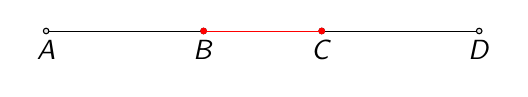
\begin{tikzpicture}
    \tkzDefPoints{0/0/A, 2/0/B, 3.5/0/C, 5.5/0/D}
    \tkzDrawSegments(A,B C,D)
    \tkzDrawPoints(A,B,C,D)
    \tkzLabelPoints[below](A,B,C,D)
    \tkzDrawPoints[color=red](B,C)
    \tkzDrawSegment[color=red](B,C)
\end{tikzpicture}
\end{minipage}
\end{tcolorbox}

\begin{example}
    Point $K$ on $\overline{ST}$ is chosen at random. What is the probability that $K$ lies on $\overline{QR}$? \bigskip 

    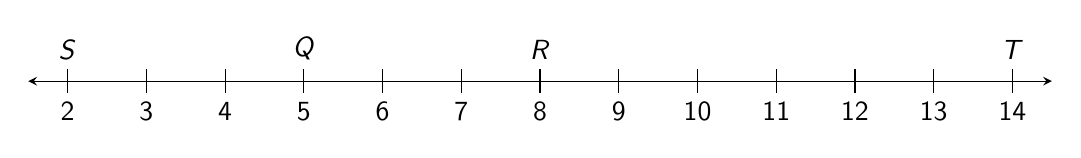
\begin{tikzpicture}
        \draw[<->] (1.5,0) -- (14.5,0);
        \foreach \x in {2,3,...,14}
        \draw (\x, 0.15) -- (\x, -0.15) node [below] {$\x$};
        \node at (2,0.15) [above] {$S$};
        \node at (5,0.15) [above] {$Q$};
        \node at (8,0.15) [above] {$R$};
        \node at (14,0.15) [above] {$T$};
    \end{tikzpicture}
\end{example}
\vspace{0.25in}

\begin{example}
    Given the diagram in the previous example, if point $H$ is randomly selected on $\overline{ST}$, what is the probability that $H$ lies on $\overline{SR}$?
\end{example}
\vspace{0.5in}

When the points of a region represent equally likely outcomes, you can find probabilities by comparing areas. \newline 

\begin{tcolorbox}[colframe=black!20!white, opacitybacktitle=0.1, coltitle=black, title=\textbf{Probability and Area}]
If point $S$ on in region $R$ is chosen at random. The probability that $S$ is in region $N$ is the ratio of the area of region $N$ to the area of region $R$. \newline 

\begin{minipage}{0.55\textwidth}
    $P(S \text{ in region } N) = \dfrac{\text{area of region } N}{\text{area of region }R}$
\end{minipage}
\begin{minipage}{0.4\textwidth}
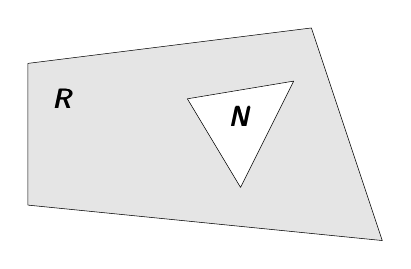
\begin{tikzpicture}[scale=0.9]
    \tkzDefPoints{0/0/A, 0/2/B, 4/2.5/C, 5/-0.5/D}
    \tkzDrawPolygon[fill=gray!20](A,B,C,D)
    \tkzDefPoints{2.25/1.5/E, 3.75/1.75/F, 3/0.25/G}
    \tkzDrawPolygon[fill=white](E,F,G)
    \node at (0.5,1.5) {$\pmb{R}$};
    \node at (3,1.25) {$\pmb{N}$};
\end{tikzpicture}
\end{minipage}
\end{tcolorbox}

\vfill 
\newpage 

\begin{example}
A point is randomly selected inside the square for each. Find the probability that it lies in the shaded region.
\begin{enumerate}[(a)]
\begin{multicols}{2}
    \item \mbox{} \newline 
    \item \mbox{} \newline 
\end{multicols}
\end{enumerate}
\begin{minipage}{0.5\textwidth}
    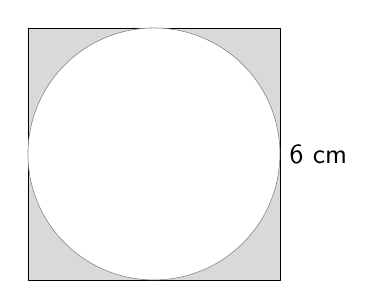
\begin{tikzpicture}[scale=0.8]
        \tkzDefPoints{0/0/O, 2/0/A, 2/2/B, -2/2/C, -2/-2/D, 2/-2/E}
        \tkzDrawPolygon[fill=gray!30](B,C,D,E)
        \tkzLabelSegment[right](B,E){6 cm}
        \tkzDrawCircle[fill=white](O,A)
    \end{tikzpicture}
\end{minipage}
\begin{minipage}{0.45\textwidth}
    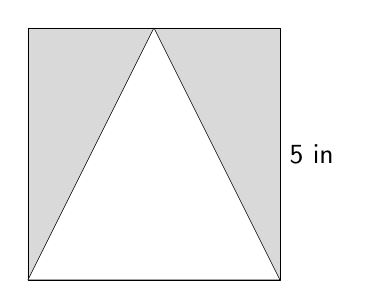
\begin{tikzpicture}[scale=0.8]
        \tkzDefPoints{0/0/A, 4/0/B, 4/4/C, 0/4/D}
        \tkzDrawPolygon[fill=gray!30](A,B,C,D)
        \tkzLabelSegment[right](B,C){5 in}
        \tkzDefMidPoint(D,C)    \tkzGetPoint{M}
        \tkzDrawPolygon[fill=white](A,M,B)
    \end{tikzpicture}
\end{minipage}
\end{example}

\vfill 

\begin{example}
An archer needs to hit the shaded area in order to win an archery contest. What is the probability that will happen? \newline

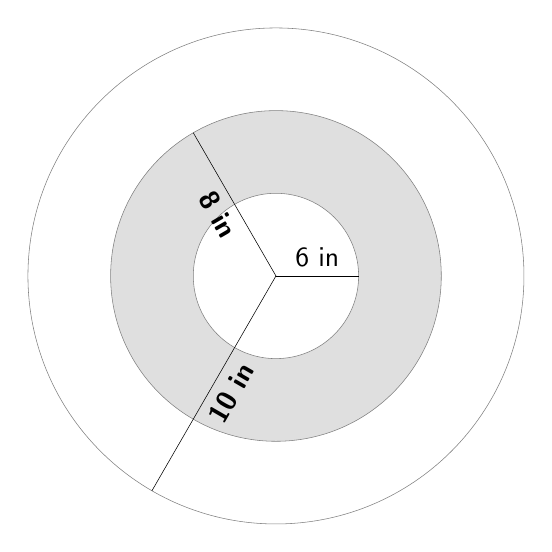
\begin{tikzpicture}[scale=0.7]
    \tkzDefPoints{0/0/O, 1.5/0/A, 3/0/B, 4.5/0/C}
    \tkzDrawCircle(O,C)
    \tkzDrawCircle[fill=gray!25](O,B)
    \tkzDrawCircle[fill=white](O,A)
    \tkzDrawSegment(O,A)
    \tkzLabelSegment[above](O,A){6 in}
    \tkzDefShiftPoint[O](120:3){D}
    \tkzDrawSegment(O,D)
    \tkzLabelSegment[sloped](O,D){\textbf{8 in}}
    \tkzDefShiftPoint[O](240:4.5){E}
    \tkzDrawSegment(O,E)
    \tkzLabelSegment[sloped](O,E){\textbf{10 in}}
\end{tikzpicture}
\end{example}

\vfill

\end{document}
